\documentclass[twoside]{book}

% Packages required by doxygen
\usepackage{calc}
\usepackage{doxygen}
\usepackage{graphicx}
\usepackage[utf8]{inputenc}
\usepackage{makeidx}
\usepackage{multicol}
\usepackage{multirow}
\usepackage{textcomp}
\usepackage[table]{xcolor}

% Font selection
\usepackage[T1]{fontenc}
\usepackage{mathptmx}
\usepackage[scaled=.90]{helvet}
\usepackage{courier}
\usepackage{amssymb}
\usepackage{sectsty}
\renewcommand{\familydefault}{\sfdefault}
\allsectionsfont{%
  \fontseries{bc}\selectfont%
  \color{darkgray}%
}
\renewcommand{\DoxyLabelFont}{%
  \fontseries{bc}\selectfont%
  \color{darkgray}%
}

% Page & text layout
\usepackage{geometry}
\geometry{%
  a4paper,%
  top=2.5cm,%
  bottom=2.5cm,%
  left=2.5cm,%
  right=2.5cm%
}
\tolerance=750
\hfuzz=15pt
\hbadness=750
\setlength{\emergencystretch}{15pt}
\setlength{\parindent}{0cm}
\setlength{\parskip}{0.2cm}
\makeatletter
\renewcommand{\paragraph}{%
  \@startsection{paragraph}{4}{0ex}{-1.0ex}{1.0ex}{%
    \normalfont\normalsize\bfseries\SS@parafont%
  }%
}
\renewcommand{\subparagraph}{%
  \@startsection{subparagraph}{5}{0ex}{-1.0ex}{1.0ex}{%
    \normalfont\normalsize\bfseries\SS@subparafont%
  }%
}
\makeatother

% Headers & footers
\usepackage{fancyhdr}
\pagestyle{fancyplain}
\fancyhead[LE]{\fancyplain{}{\bfseries\thepage}}
\fancyhead[CE]{\fancyplain{}{}}
\fancyhead[RE]{\fancyplain{}{\bfseries\leftmark}}
\fancyhead[LO]{\fancyplain{}{\bfseries\rightmark}}
\fancyhead[CO]{\fancyplain{}{}}
\fancyhead[RO]{\fancyplain{}{\bfseries\thepage}}
\fancyfoot[LE]{\fancyplain{}{}}
\fancyfoot[CE]{\fancyplain{}{}}
\fancyfoot[RE]{\fancyplain{}{\bfseries\scriptsize Generated on Mon May 2 2016 23\-:47\-:35 for My Project by Doxygen }}
\fancyfoot[LO]{\fancyplain{}{\bfseries\scriptsize Generated on Mon May 2 2016 23\-:47\-:35 for My Project by Doxygen }}
\fancyfoot[CO]{\fancyplain{}{}}
\fancyfoot[RO]{\fancyplain{}{}}
\renewcommand{\footrulewidth}{0.4pt}
\renewcommand{\chaptermark}[1]{%
  \markboth{#1}{}%
}
\renewcommand{\sectionmark}[1]{%
  \markright{\thesection\ #1}%
}

% Indices & bibliography
\usepackage{natbib}
\usepackage[titles]{tocloft}
\setcounter{tocdepth}{3}
\setcounter{secnumdepth}{5}
\makeindex

% Hyperlinks (required, but should be loaded last)
\usepackage{ifpdf}
\ifpdf
  \usepackage[pdftex,pagebackref=true]{hyperref}
\else
  \usepackage[ps2pdf,pagebackref=true]{hyperref}
\fi
\hypersetup{%
  colorlinks=true,%
  linkcolor=blue,%
  citecolor=blue,%
  unicode%
}

% Custom commands
\newcommand{\clearemptydoublepage}{%
  \newpage{\pagestyle{empty}\cleardoublepage}%
}


%===== C O N T E N T S =====

\begin{document}

% Titlepage & ToC
\hypersetup{pageanchor=false}
\pagenumbering{roman}
\begin{titlepage}
\vspace*{7cm}
\begin{center}%
{\Large My Project }\\
\vspace*{1cm}
{\large Generated by Doxygen 1.8.5}\\
\vspace*{0.5cm}
{\small Mon May 2 2016 23:47:35}\\
\end{center}
\end{titlepage}
\clearemptydoublepage
\tableofcontents
\clearemptydoublepage
\pagenumbering{arabic}
\hypersetup{pageanchor=true}

%--- Begin generated contents ---
\chapter{Hierarchical Index}
\section{Class Hierarchy}
This inheritance list is sorted roughly, but not completely, alphabetically\-:\begin{DoxyCompactList}
\item \contentsline{section}{Boid}{\pageref{classBoid}}{}
\item \contentsline{section}{Boid\-Math}{\pageref{classBoidMath}}{}
\item \contentsline{section}{Octree}{\pageref{classOctree}}{}
\item Q\-G\-L\-Widget\begin{DoxyCompactList}
\item \contentsline{section}{N\-G\-L\-Scene}{\pageref{classNGLScene}}{}
\end{DoxyCompactList}
\item Q\-Main\-Window\begin{DoxyCompactList}
\item \contentsline{section}{Main\-Window}{\pageref{classMainWindow}}{}
\end{DoxyCompactList}
\item \contentsline{section}{Swarm}{\pageref{classSwarm}}{}
\end{DoxyCompactList}

\chapter{Class Index}
\section{Class List}
Here are the classes, structs, unions and interfaces with brief descriptions\-:\begin{DoxyCompactList}
\item\contentsline{section}{\hyperlink{classBoid}{Boid} \\*This class contains movement methods and behaviours for the boids }{\pageref{classBoid}}{}
\item\contentsline{section}{\hyperlink{classBoidMath}{Boid\-Math} \\*This class calculates the distance between the boids }{\pageref{classBoidMath}}{}
\item\contentsline{section}{\hyperlink{classMainWindow}{Main\-Window} \\*This class connects G\-U\-I with \hyperlink{classNGLScene}{N\-G\-L\-Scene} }{\pageref{classMainWindow}}{}
\item\contentsline{section}{\hyperlink{classNGLScene}{N\-G\-L\-Scene} \\*This class draws all elements for the swarming simulation }{\pageref{classNGLScene}}{}
\item\contentsline{section}{\hyperlink{classOctree}{Octree} \\*I have used this class for finding the neighbours of a boid in my swarming system. I have made small modification from the original class such as removing methods which were not necesarrily needed for the calculations }{\pageref{classOctree}}{}
\item\contentsline{section}{\hyperlink{classSwarm}{Swarm} \\*Class for creating the swarm, managing boids and their neighbours }{\pageref{classSwarm}}{}
\end{DoxyCompactList}

\chapter{File Index}
\section{File List}
Here is a list of all documented files with brief descriptions\-:\begin{DoxyCompactList}
\item\contentsline{section}{include/\hyperlink{Boid_8h}{Boid.\-h} }{\pageref{Boid_8h}}{}
\item\contentsline{section}{include/\hyperlink{BoidMath_8h}{Boid\-Math.\-h} }{\pageref{BoidMath_8h}}{}
\item\contentsline{section}{include/\hyperlink{MainWindow_8h}{Main\-Window.\-h} }{\pageref{MainWindow_8h}}{}
\item\contentsline{section}{include/\hyperlink{NGLScene_8h}{N\-G\-L\-Scene.\-h} \\*Basic Qt G\-L window class for creating a swarming simulation }{\pageref{NGLScene_8h}}{}
\item\contentsline{section}{include/\hyperlink{Octree_8h}{Octree.\-h} }{\pageref{Octree_8h}}{}
\item\contentsline{section}{include/\hyperlink{Swarm_8h}{Swarm.\-h} }{\pageref{Swarm_8h}}{}
\end{DoxyCompactList}

\chapter{Class Documentation}
\hypertarget{classBoid}{\section{Boid Class Reference}
\label{classBoid}\index{Boid@{Boid}}
}


this class contains movement methods and behaviours for the boids  




{\ttfamily \#include $<$Boid.\-h$>$}

\subsection*{Public Member Functions}
\begin{DoxyCompactItemize}
\item 
\hyperlink{classBoid_a5d1abb62ea2b9f7adc764d648614bf51}{Boid} (int \-\_\-id)
\begin{DoxyCompactList}\small\item\em ctor \end{DoxyCompactList}\item 
\hypertarget{classBoid_a712f84ddc1b8ad06ad7ecd6c10a1666c}{\hyperlink{classBoid_a712f84ddc1b8ad06ad7ecd6c10a1666c}{$\sim$\-Boid} ()}\label{classBoid_a712f84ddc1b8ad06ad7ecd6c10a1666c}

\begin{DoxyCompactList}\small\item\em dtor \end{DoxyCompactList}\item 
void \hyperlink{classBoid_a38026ec733e0e7e705127e3f88f69b99}{set\-Pos} (float \-\_\-x, float \-\_\-y, float \-\_\-z)
\begin{DoxyCompactList}\small\item\em method to st the boid position \end{DoxyCompactList}\item 
void \hyperlink{classBoid_a97552481a8c6f43e203d0bc2df083830}{set\-Neighbour} (\hyperlink{classBoid}{Boid} $\ast$boid)
\begin{DoxyCompactList}\small\item\em method to set a neighbour to the boid \end{DoxyCompactList}\item 
void \hyperlink{classBoid_aeb1fd57777cec9eab3f735312c2a2599}{clear\-Neighbour} ()
\begin{DoxyCompactList}\small\item\em method to cclear the boid's neighbours \end{DoxyCompactList}\item 
void \hyperlink{classBoid_a610fd5764690285c3c81135c30162633}{set\-Velocity} (float \-\_\-x, float \-\_\-y, float \-\_\-z)
\begin{DoxyCompactList}\small\item\em method to set the boid's velocity \end{DoxyCompactList}\item 
void \hyperlink{classBoid_af24205fb4e30e0e746c3146c59252fda}{set\-S\-Weight} (int \-\_\-separation\-Weight)
\begin{DoxyCompactList}\small\item\em method to set the weight on the separation force \end{DoxyCompactList}\item 
void \hyperlink{classBoid_aa2ace7fb25c823079ebdab97dfefdf28}{set\-C\-Weight} (int \-\_\-cohesion\-Weight)
\begin{DoxyCompactList}\small\item\em method to set the weight on the cohesion force \end{DoxyCompactList}\item 
void \hyperlink{classBoid_acc3767ea7aaff905b618aab1dcb8d2e3}{set\-A\-Weight} (int \-\_\-align\-Weight)
\begin{DoxyCompactList}\small\item\em method to set the weight on the alignment force \end{DoxyCompactList}\item 
void \hyperlink{classBoid_af9cc5ca3786b7a0c5fa7c6b61d257bde}{set\-Mass} (int \-\_\-mass)
\begin{DoxyCompactList}\small\item\em method to set the mass of the boid \end{DoxyCompactList}\item 
void \hyperlink{classBoid_a6a8b730efcf6b98cbf56aaa905bc7508}{set\-Speed} (float \-\_\-speed)
\begin{DoxyCompactList}\small\item\em method to set the speed of the boid \end{DoxyCompactList}\item 
void \hyperlink{classBoid_a8b2d2ef70003c3b46c22ec3866f842ec}{set\-Sep\-Dist} (int \-\_\-sep\-Dist)
\begin{DoxyCompactList}\small\item\em method to set the separation distance \end{DoxyCompactList}\item 
int \hyperlink{classBoid_ae4d6cb62f1811008b923e1d1bf349430}{get\-Neighbours} () const 
\begin{DoxyCompactList}\small\item\em method to get the number of neighbours the boid has \end{DoxyCompactList}\item 
ngl\-::\-Vec3 \hyperlink{classBoid_a8d92ae43f4b135661bb93afd46c90e94}{get\-Position} () const 
\begin{DoxyCompactList}\small\item\em method to get the position of the boid \end{DoxyCompactList}\item 
ngl\-::\-Vec3 \hyperlink{classBoid_a9b8109fd5bb93268c2591bf0b87a920d}{get\-Velocity} () const 
\begin{DoxyCompactList}\small\item\em method to get the velocity of the boid \end{DoxyCompactList}\item 
\hypertarget{classBoid_a5ff5c09aa0f501a097116a453013986f}{float {\bfseries get\-Radius} () const }\label{classBoid_a5ff5c09aa0f501a097116a453013986f}

\item 
int \hyperlink{classBoid_a579520e335b6033643531218eae95be0}{get\-Id} () const 
\begin{DoxyCompactList}\small\item\em method to get the id of a boid \end{DoxyCompactList}\item 
ngl\-::\-Vec3 \hyperlink{classBoid_aef5f32444ae2ae6fff812cb8272e437f}{get\-Rotation} () const 
\begin{DoxyCompactList}\small\item\em method to get the x and y rotations of a boid \end{DoxyCompactList}\item 
int \hyperlink{classBoid_ab474ff0fa3273519a0284bda734d7119}{get\-Search\-Rad} () const 
\begin{DoxyCompactList}\small\item\em method to get the distance a boid will look for neighbours \end{DoxyCompactList}\item 
\hypertarget{classBoid_aa2b619d85612051c88b2e7cc67ac0115}{void \hyperlink{classBoid_aa2b619d85612051c88b2e7cc67ac0115}{set\-Steering} ()}\label{classBoid_aa2b619d85612051c88b2e7cc67ac0115}

\begin{DoxyCompactList}\small\item\em method to calculate and set steering force vector \end{DoxyCompactList}\item 
\hypertarget{classBoid_af0fb09a2a09da233530c37466ca1e2f2}{void \hyperlink{classBoid_af0fb09a2a09da233530c37466ca1e2f2}{set\-Cohesion} ()}\label{classBoid_af0fb09a2a09da233530c37466ca1e2f2}

\begin{DoxyCompactList}\small\item\em method to calculate and set cohesion force vector \end{DoxyCompactList}\item 
\hypertarget{classBoid_a6f14922235fdd42e64a0b462113d3f16}{void \hyperlink{classBoid_a6f14922235fdd42e64a0b462113d3f16}{set\-Alignment} ()}\label{classBoid_a6f14922235fdd42e64a0b462113d3f16}

\begin{DoxyCompactList}\small\item\em method to calculate and set the alignment force vector \end{DoxyCompactList}\item 
\hypertarget{classBoid_af68e960efe0425045524acf58d681ffb}{void \hyperlink{classBoid_af68e960efe0425045524acf58d681ffb}{set\-Separation} ()}\label{classBoid_af68e960efe0425045524acf58d681ffb}

\begin{DoxyCompactList}\small\item\em method to calculate and set the separation force vector \end{DoxyCompactList}\item 
\hypertarget{classBoid_add0e553d230a21b35c6e60d8af5f4b9a}{void \hyperlink{classBoid_add0e553d230a21b35c6e60d8af5f4b9a}{set\-Avoid} ()}\label{classBoid_add0e553d230a21b35c6e60d8af5f4b9a}

\begin{DoxyCompactList}\small\item\em method to calculate and set the avoidance force vector \end{DoxyCompactList}\item 
void \hyperlink{classBoid_abaf050c8e4f90b41bacaa4ae850d9722}{set\-Reposition} (ngl\-::\-Vec3 \-\_\-reposition)
\begin{DoxyCompactList}\small\item\em method to calculate and set the reposition force vector \end{DoxyCompactList}\item 
\hypertarget{classBoid_abc245a74a8c5e124ba98d0d07c5ab01e}{void \hyperlink{classBoid_abc245a74a8c5e124ba98d0d07c5ab01e}{reposition\-Bounds} ()}\label{classBoid_abc245a74a8c5e124ba98d0d07c5ab01e}

\begin{DoxyCompactList}\small\item\em method to calculate and set the reposition force vector away from the walls of the \hyperlink{classSwarm}{Swarm} \end{DoxyCompactList}\item 
\hypertarget{classBoid_a141b020067545d3c3af45e26084d257f}{void {\bfseries set\-Direction} ()}\label{classBoid_a141b020067545d3c3af45e26084d257f}

\item 
\hypertarget{classBoid_a9133cb1a761dbbd80a535b4f5576dd00}{void \hyperlink{classBoid_a9133cb1a761dbbd80a535b4f5576dd00}{update\-Position} ()}\label{classBoid_a9133cb1a761dbbd80a535b4f5576dd00}

\begin{DoxyCompactList}\small\item\em method to calculate and set the new position based on the current steering vector, current velocity and speed \end{DoxyCompactList}\item 
\hypertarget{classBoid_ad84ed9152d035b542921547f289024eb}{void \hyperlink{classBoid_ad84ed9152d035b542921547f289024eb}{move} ()}\label{classBoid_ad84ed9152d035b542921547f289024eb}

\begin{DoxyCompactList}\small\item\em method to move the boid by combining all the steering methods and update\-Position \end{DoxyCompactList}\item 
\hypertarget{classBoid_a03d008ad343ad4a7d2c6d3ba3c6556ee}{void \hyperlink{classBoid_a03d008ad343ad4a7d2c6d3ba3c6556ee}{set\-Rotate} ()}\label{classBoid_a03d008ad343ad4a7d2c6d3ba3c6556ee}

\begin{DoxyCompactList}\small\item\em method to calculate and set the boid's rotation based on its velocity \end{DoxyCompactList}\item 
\hypertarget{classBoid_a145b410db5f17eb0896ee48baa769a1c}{void \hyperlink{classBoid_a145b410db5f17eb0896ee48baa769a1c}{Collision} (ngl\-::\-Vec3 \-\_\-pos, float \-\_\-rad)}\label{classBoid_a145b410db5f17eb0896ee48baa769a1c}

\begin{DoxyCompactList}\small\item\em method to check if boids are colliding \end{DoxyCompactList}\end{DoxyCompactItemize}


\subsection{Detailed Description}
this class contains movement methods and behaviours for the boids 

\subsection{Constructor \& Destructor Documentation}
\hypertarget{classBoid_a5d1abb62ea2b9f7adc764d648614bf51}{\index{Boid@{Boid}!Boid@{Boid}}
\index{Boid@{Boid}!Boid@{Boid}}
\subsubsection[{Boid}]{\setlength{\rightskip}{0pt plus 5cm}Boid\-::\-Boid (
\begin{DoxyParamCaption}
\item[{int}]{\-\_\-id}
\end{DoxyParamCaption}
)}}\label{classBoid_a5d1abb62ea2b9f7adc764d648614bf51}


ctor 


\begin{DoxyParams}[1]{Parameters}
\mbox{\tt in}  & {\em \-\_\-id} & boid I\-D \\
\hline
\end{DoxyParams}


\subsection{Member Function Documentation}
\hypertarget{classBoid_aeb1fd57777cec9eab3f735312c2a2599}{\index{Boid@{Boid}!clear\-Neighbour@{clear\-Neighbour}}
\index{clear\-Neighbour@{clear\-Neighbour}!Boid@{Boid}}
\subsubsection[{clear\-Neighbour}]{\setlength{\rightskip}{0pt plus 5cm}void Boid\-::clear\-Neighbour (
\begin{DoxyParamCaption}
{}
\end{DoxyParamCaption}
)}}\label{classBoid_aeb1fd57777cec9eab3f735312c2a2599}


method to cclear the boid's neighbours 

\begin{DoxyReturn}{Returns}
clears m\-\_\-neighbours 
\end{DoxyReturn}
\hypertarget{classBoid_a579520e335b6033643531218eae95be0}{\index{Boid@{Boid}!get\-Id@{get\-Id}}
\index{get\-Id@{get\-Id}!Boid@{Boid}}
\subsubsection[{get\-Id}]{\setlength{\rightskip}{0pt plus 5cm}int Boid\-::get\-Id (
\begin{DoxyParamCaption}
{}
\end{DoxyParamCaption}
) const\hspace{0.3cm}{\ttfamily [inline]}}}\label{classBoid_a579520e335b6033643531218eae95be0}


method to get the id of a boid 

\begin{DoxyReturn}{Returns}
returns m\-\_\-id 
\end{DoxyReturn}
\hypertarget{classBoid_ae4d6cb62f1811008b923e1d1bf349430}{\index{Boid@{Boid}!get\-Neighbours@{get\-Neighbours}}
\index{get\-Neighbours@{get\-Neighbours}!Boid@{Boid}}
\subsubsection[{get\-Neighbours}]{\setlength{\rightskip}{0pt plus 5cm}int Boid\-::get\-Neighbours (
\begin{DoxyParamCaption}
{}
\end{DoxyParamCaption}
) const\hspace{0.3cm}{\ttfamily [inline]}}}\label{classBoid_ae4d6cb62f1811008b923e1d1bf349430}


method to get the number of neighbours the boid has 

\begin{DoxyReturn}{Returns}
returns the size of m\-\_\-neighbours 
\end{DoxyReturn}
\hypertarget{classBoid_a8d92ae43f4b135661bb93afd46c90e94}{\index{Boid@{Boid}!get\-Position@{get\-Position}}
\index{get\-Position@{get\-Position}!Boid@{Boid}}
\subsubsection[{get\-Position}]{\setlength{\rightskip}{0pt plus 5cm}ngl\-::\-Vec3 Boid\-::get\-Position (
\begin{DoxyParamCaption}
{}
\end{DoxyParamCaption}
) const\hspace{0.3cm}{\ttfamily [inline]}}}\label{classBoid_a8d92ae43f4b135661bb93afd46c90e94}


method to get the position of the boid 

\begin{DoxyReturn}{Returns}
returns m\-\_\-position 
\end{DoxyReturn}
\hypertarget{classBoid_aef5f32444ae2ae6fff812cb8272e437f}{\index{Boid@{Boid}!get\-Rotation@{get\-Rotation}}
\index{get\-Rotation@{get\-Rotation}!Boid@{Boid}}
\subsubsection[{get\-Rotation}]{\setlength{\rightskip}{0pt plus 5cm}ngl\-::\-Vec3 Boid\-::get\-Rotation (
\begin{DoxyParamCaption}
{}
\end{DoxyParamCaption}
) const\hspace{0.3cm}{\ttfamily [inline]}}}\label{classBoid_aef5f32444ae2ae6fff812cb8272e437f}


method to get the x and y rotations of a boid 

\begin{DoxyReturn}{Returns}
returns a Vec3 of (m\-\_\-pitch, m\-\_\-yaw, 0) 
\end{DoxyReturn}
\hypertarget{classBoid_ab474ff0fa3273519a0284bda734d7119}{\index{Boid@{Boid}!get\-Search\-Rad@{get\-Search\-Rad}}
\index{get\-Search\-Rad@{get\-Search\-Rad}!Boid@{Boid}}
\subsubsection[{get\-Search\-Rad}]{\setlength{\rightskip}{0pt plus 5cm}int Boid\-::get\-Search\-Rad (
\begin{DoxyParamCaption}
{}
\end{DoxyParamCaption}
) const\hspace{0.3cm}{\ttfamily [inline]}}}\label{classBoid_ab474ff0fa3273519a0284bda734d7119}


method to get the distance a boid will look for neighbours 

\begin{DoxyReturn}{Returns}
returns m\-\_\-search\-Rad 
\end{DoxyReturn}
\hypertarget{classBoid_a9b8109fd5bb93268c2591bf0b87a920d}{\index{Boid@{Boid}!get\-Velocity@{get\-Velocity}}
\index{get\-Velocity@{get\-Velocity}!Boid@{Boid}}
\subsubsection[{get\-Velocity}]{\setlength{\rightskip}{0pt plus 5cm}ngl\-::\-Vec3 Boid\-::get\-Velocity (
\begin{DoxyParamCaption}
{}
\end{DoxyParamCaption}
) const\hspace{0.3cm}{\ttfamily [inline]}}}\label{classBoid_a9b8109fd5bb93268c2591bf0b87a920d}


method to get the velocity of the boid 

\begin{DoxyReturn}{Returns}
returns m\-\_\-velocity 
\end{DoxyReturn}
\hypertarget{classBoid_acc3767ea7aaff905b618aab1dcb8d2e3}{\index{Boid@{Boid}!set\-A\-Weight@{set\-A\-Weight}}
\index{set\-A\-Weight@{set\-A\-Weight}!Boid@{Boid}}
\subsubsection[{set\-A\-Weight}]{\setlength{\rightskip}{0pt plus 5cm}void Boid\-::set\-A\-Weight (
\begin{DoxyParamCaption}
\item[{int}]{\-\_\-align\-Weight}
\end{DoxyParamCaption}
)}}\label{classBoid_acc3767ea7aaff905b618aab1dcb8d2e3}


method to set the weight on the alignment force 


\begin{DoxyParams}[1]{Parameters}
\mbox{\tt in}  & {\em \-\_\-align\-Weight} & the weight value to set \\
\hline
\end{DoxyParams}
\hypertarget{classBoid_aa2ace7fb25c823079ebdab97dfefdf28}{\index{Boid@{Boid}!set\-C\-Weight@{set\-C\-Weight}}
\index{set\-C\-Weight@{set\-C\-Weight}!Boid@{Boid}}
\subsubsection[{set\-C\-Weight}]{\setlength{\rightskip}{0pt plus 5cm}void Boid\-::set\-C\-Weight (
\begin{DoxyParamCaption}
\item[{int}]{\-\_\-cohesion\-Weight}
\end{DoxyParamCaption}
)}}\label{classBoid_aa2ace7fb25c823079ebdab97dfefdf28}


method to set the weight on the cohesion force 


\begin{DoxyParams}[1]{Parameters}
\mbox{\tt in}  & {\em \-\_\-cohesion\-Weight} & the weight value to set \\
\hline
\end{DoxyParams}
\hypertarget{classBoid_af9cc5ca3786b7a0c5fa7c6b61d257bde}{\index{Boid@{Boid}!set\-Mass@{set\-Mass}}
\index{set\-Mass@{set\-Mass}!Boid@{Boid}}
\subsubsection[{set\-Mass}]{\setlength{\rightskip}{0pt plus 5cm}void Boid\-::set\-Mass (
\begin{DoxyParamCaption}
\item[{int}]{\-\_\-mass}
\end{DoxyParamCaption}
)}}\label{classBoid_af9cc5ca3786b7a0c5fa7c6b61d257bde}


method to set the mass of the boid 


\begin{DoxyParams}[1]{Parameters}
\mbox{\tt in}  & {\em \-\_\-mass} & the value to set \\
\hline
\end{DoxyParams}
\hypertarget{classBoid_a97552481a8c6f43e203d0bc2df083830}{\index{Boid@{Boid}!set\-Neighbour@{set\-Neighbour}}
\index{set\-Neighbour@{set\-Neighbour}!Boid@{Boid}}
\subsubsection[{set\-Neighbour}]{\setlength{\rightskip}{0pt plus 5cm}void Boid\-::set\-Neighbour (
\begin{DoxyParamCaption}
\item[{{\bf Boid} $\ast$}]{boid}
\end{DoxyParamCaption}
)}}\label{classBoid_a97552481a8c6f43e203d0bc2df083830}


method to set a neighbour to the boid 


\begin{DoxyParams}[1]{Parameters}
\mbox{\tt in}  & {\em boid} & the neighbouring boid \\
\hline
\end{DoxyParams}
\begin{DoxyReturn}{Returns}
appends boid to m\-\_\-neighbours 
\end{DoxyReturn}
\hypertarget{classBoid_a38026ec733e0e7e705127e3f88f69b99}{\index{Boid@{Boid}!set\-Pos@{set\-Pos}}
\index{set\-Pos@{set\-Pos}!Boid@{Boid}}
\subsubsection[{set\-Pos}]{\setlength{\rightskip}{0pt plus 5cm}void Boid\-::set\-Pos (
\begin{DoxyParamCaption}
\item[{float}]{\-\_\-x, }
\item[{float}]{\-\_\-y, }
\item[{float}]{\-\_\-z}
\end{DoxyParamCaption}
)}}\label{classBoid_a38026ec733e0e7e705127e3f88f69b99}


method to st the boid position 


\begin{DoxyParams}[1]{Parameters}
\mbox{\tt in}  & {\em \-\_\-x} & the x value ot be set \\
\hline
\mbox{\tt in}  & {\em \-\_\-y} & the y value ot be set \\
\hline
\mbox{\tt in}  & {\em \-\_\-z} & the z value ot be set \\
\hline
\end{DoxyParams}
\hypertarget{classBoid_abaf050c8e4f90b41bacaa4ae850d9722}{\index{Boid@{Boid}!set\-Reposition@{set\-Reposition}}
\index{set\-Reposition@{set\-Reposition}!Boid@{Boid}}
\subsubsection[{set\-Reposition}]{\setlength{\rightskip}{0pt plus 5cm}void Boid\-::set\-Reposition (
\begin{DoxyParamCaption}
\item[{ngl\-::\-Vec3}]{\-\_\-reposition}
\end{DoxyParamCaption}
)}}\label{classBoid_abaf050c8e4f90b41bacaa4ae850d9722}


method to calculate and set the reposition force vector 


\begin{DoxyParams}[1]{Parameters}
\mbox{\tt in}  & {\em \-\_\-reposition} & the point to reposition from \\
\hline
\end{DoxyParams}
\hypertarget{classBoid_a8b2d2ef70003c3b46c22ec3866f842ec}{\index{Boid@{Boid}!set\-Sep\-Dist@{set\-Sep\-Dist}}
\index{set\-Sep\-Dist@{set\-Sep\-Dist}!Boid@{Boid}}
\subsubsection[{set\-Sep\-Dist}]{\setlength{\rightskip}{0pt plus 5cm}void Boid\-::set\-Sep\-Dist (
\begin{DoxyParamCaption}
\item[{int}]{\-\_\-sep\-Dist}
\end{DoxyParamCaption}
)\hspace{0.3cm}{\ttfamily [inline]}}}\label{classBoid_a8b2d2ef70003c3b46c22ec3866f842ec}


method to set the separation distance 


\begin{DoxyParams}[1]{Parameters}
\mbox{\tt in}  & {\em \-\_\-sep\-Dist} & the value to be set \\
\hline
\end{DoxyParams}
\hypertarget{classBoid_a6a8b730efcf6b98cbf56aaa905bc7508}{\index{Boid@{Boid}!set\-Speed@{set\-Speed}}
\index{set\-Speed@{set\-Speed}!Boid@{Boid}}
\subsubsection[{set\-Speed}]{\setlength{\rightskip}{0pt plus 5cm}void Boid\-::set\-Speed (
\begin{DoxyParamCaption}
\item[{float}]{\-\_\-speed}
\end{DoxyParamCaption}
)}}\label{classBoid_a6a8b730efcf6b98cbf56aaa905bc7508}


method to set the speed of the boid 


\begin{DoxyParams}{Parameters}
{\em \-\_\-speed} & the speed value to set \\
\hline
\end{DoxyParams}
\hypertarget{classBoid_af24205fb4e30e0e746c3146c59252fda}{\index{Boid@{Boid}!set\-S\-Weight@{set\-S\-Weight}}
\index{set\-S\-Weight@{set\-S\-Weight}!Boid@{Boid}}
\subsubsection[{set\-S\-Weight}]{\setlength{\rightskip}{0pt plus 5cm}void Boid\-::set\-S\-Weight (
\begin{DoxyParamCaption}
\item[{int}]{\-\_\-separation\-Weight}
\end{DoxyParamCaption}
)}}\label{classBoid_af24205fb4e30e0e746c3146c59252fda}


method to set the weight on the separation force 


\begin{DoxyParams}[1]{Parameters}
\mbox{\tt in}  & {\em \-\_\-separation\-Weight} & the weight value to set \\
\hline
\end{DoxyParams}
\hypertarget{classBoid_a610fd5764690285c3c81135c30162633}{\index{Boid@{Boid}!set\-Velocity@{set\-Velocity}}
\index{set\-Velocity@{set\-Velocity}!Boid@{Boid}}
\subsubsection[{set\-Velocity}]{\setlength{\rightskip}{0pt plus 5cm}void Boid\-::set\-Velocity (
\begin{DoxyParamCaption}
\item[{float}]{\-\_\-x, }
\item[{float}]{\-\_\-y, }
\item[{float}]{\-\_\-z}
\end{DoxyParamCaption}
)}}\label{classBoid_a610fd5764690285c3c81135c30162633}


method to set the boid's velocity 


\begin{DoxyParams}[1]{Parameters}
\mbox{\tt in}  & {\em \-\_\-x} & the x value ot be set \\
\hline
\mbox{\tt in}  & {\em \-\_\-y} & the y value ot be set \\
\hline
\mbox{\tt in}  & {\em \-\_\-z} & the z value ot be set \\
\hline
\end{DoxyParams}


The documentation for this class was generated from the following files\-:\begin{DoxyCompactItemize}
\item 
include/\hyperlink{Boid_8h}{Boid.\-h}\item 
src/Boid.\-cpp\end{DoxyCompactItemize}

\hypertarget{classBoidMath}{\section{Boid\-Math Class Reference}
\label{classBoidMath}\index{Boid\-Math@{Boid\-Math}}
}


this class calculates the distance between the boids  




{\ttfamily \#include $<$Boid\-Math.\-h$>$}

\subsection*{Public Member Functions}
\begin{DoxyCompactItemize}
\item 
\hyperlink{classBoidMath_a96f701b19a18f2a07372f5eb50548e99}{Boid\-Math} ()
\begin{DoxyCompactList}\small\item\em ctor \end{DoxyCompactList}\item 
\hyperlink{classBoidMath_a1b7dfa1c968c08d4ed9ba03be75d91e0}{$\sim$\-Boid\-Math} ()
\begin{DoxyCompactList}\small\item\em ctor \end{DoxyCompactList}\end{DoxyCompactItemize}
\subsection*{Static Public Member Functions}
\begin{DoxyCompactItemize}
\item 
static float \hyperlink{classBoidMath_a1aaae5ede2b0287d2426a7a8d86adbd2}{distance} (ngl\-::\-Vec3 a, ngl\-::\-Vec3 b)
\begin{DoxyCompactList}\small\item\em method to calculate the distance between the boids in the swarm \end{DoxyCompactList}\item 
\hypertarget{classBoidMath_a555606e357d0021da57236ad97656d86}{static bool \hyperlink{classBoidMath_a555606e357d0021da57236ad97656d86}{collision\-Detect} (ngl\-::\-Vec3 ahead, ngl\-::\-Vec3 a, ngl\-::\-Vec3 b, float radius)}\label{classBoidMath_a555606e357d0021da57236ad97656d86}

\begin{DoxyCompactList}\small\item\em method to calculate detect if a collision has occured \end{DoxyCompactList}\item 
static bool \hyperlink{classBoidMath_a10348823145de6823516c6a78df0075d}{box\-Intersects\-Sphere} (ngl\-::\-Vec3 b\-Min, ngl\-::\-Vec3 b\-Max, ngl\-::\-Vec3 C, float r)
\begin{DoxyCompactList}\small\item\em query if a box intersects with a sphere \end{DoxyCompactList}\end{DoxyCompactItemize}


\subsection{Detailed Description}
this class calculates the distance between the boids 

\subsection{Constructor \& Destructor Documentation}
\hypertarget{classBoidMath_a96f701b19a18f2a07372f5eb50548e99}{\index{Boid\-Math@{Boid\-Math}!Boid\-Math@{Boid\-Math}}
\index{Boid\-Math@{Boid\-Math}!BoidMath@{Boid\-Math}}
\subsubsection[{Boid\-Math}]{\setlength{\rightskip}{0pt plus 5cm}Boid\-Math\-::\-Boid\-Math (
\begin{DoxyParamCaption}
{}
\end{DoxyParamCaption}
)}}\label{classBoidMath_a96f701b19a18f2a07372f5eb50548e99}


ctor 

ctr \hypertarget{classBoidMath_a1b7dfa1c968c08d4ed9ba03be75d91e0}{\index{Boid\-Math@{Boid\-Math}!$\sim$\-Boid\-Math@{$\sim$\-Boid\-Math}}
\index{$\sim$\-Boid\-Math@{$\sim$\-Boid\-Math}!BoidMath@{Boid\-Math}}
\subsubsection[{$\sim$\-Boid\-Math}]{\setlength{\rightskip}{0pt plus 5cm}Boid\-Math\-::$\sim$\-Boid\-Math (
\begin{DoxyParamCaption}
{}
\end{DoxyParamCaption}
)}}\label{classBoidMath_a1b7dfa1c968c08d4ed9ba03be75d91e0}


ctor 

dtr 

\subsection{Member Function Documentation}
\hypertarget{classBoidMath_a10348823145de6823516c6a78df0075d}{\index{Boid\-Math@{Boid\-Math}!box\-Intersects\-Sphere@{box\-Intersects\-Sphere}}
\index{box\-Intersects\-Sphere@{box\-Intersects\-Sphere}!BoidMath@{Boid\-Math}}
\subsubsection[{box\-Intersects\-Sphere}]{\setlength{\rightskip}{0pt plus 5cm}bool Boid\-Math\-::box\-Intersects\-Sphere (
\begin{DoxyParamCaption}
\item[{ngl\-::\-Vec3}]{b\-Min, }
\item[{ngl\-::\-Vec3}]{b\-Max, }
\item[{ngl\-::\-Vec3}]{C, }
\item[{float}]{r}
\end{DoxyParamCaption}
)\hspace{0.3cm}{\ttfamily [static]}}}\label{classBoidMath_a10348823145de6823516c6a78df0075d}


query if a box intersects with a sphere 


\begin{DoxyParams}[1]{Parameters}
\mbox{\tt in}  & {\em b\-Min} & the minimum corner of the box \\
\hline
\mbox{\tt in}  & {\em b\-Max} & the maximum corner of the box \\
\hline
\mbox{\tt in}  & {\em C} & the centre of the sphere \\
\hline
\mbox{\tt in}  & {\em r} & the radius of the circle \\
\hline
\end{DoxyParams}
\begin{DoxyReturn}{Returns}
true if box intersects with sphere, false if not 
\end{DoxyReturn}
\hypertarget{classBoidMath_a1aaae5ede2b0287d2426a7a8d86adbd2}{\index{Boid\-Math@{Boid\-Math}!distance@{distance}}
\index{distance@{distance}!BoidMath@{Boid\-Math}}
\subsubsection[{distance}]{\setlength{\rightskip}{0pt plus 5cm}float Boid\-Math\-::distance (
\begin{DoxyParamCaption}
\item[{ngl\-::\-Vec3}]{a, }
\item[{ngl\-::\-Vec3}]{b}
\end{DoxyParamCaption}
)\hspace{0.3cm}{\ttfamily [static]}}}\label{classBoidMath_a1aaae5ede2b0287d2426a7a8d86adbd2}


method to calculate the distance between the boids in the swarm 

calculate the magnitude/distance between two points to determine collision or if a neighbour is within radius of boid 

The documentation for this class was generated from the following files\-:\begin{DoxyCompactItemize}
\item 
include/\hyperlink{BoidMath_8h}{Boid\-Math.\-h}\item 
src/Boidmath.\-cpp\end{DoxyCompactItemize}

\hypertarget{classMainWindow}{\section{Main\-Window Class Reference}
\label{classMainWindow}\index{Main\-Window@{Main\-Window}}
}


this class connects G\-U\-I with \hyperlink{classNGLScene}{N\-G\-L\-Scene}  




{\ttfamily \#include $<$Main\-Window.\-h$>$}

Inheritance diagram for Main\-Window\-:\begin{figure}[H]
\begin{center}
\leavevmode
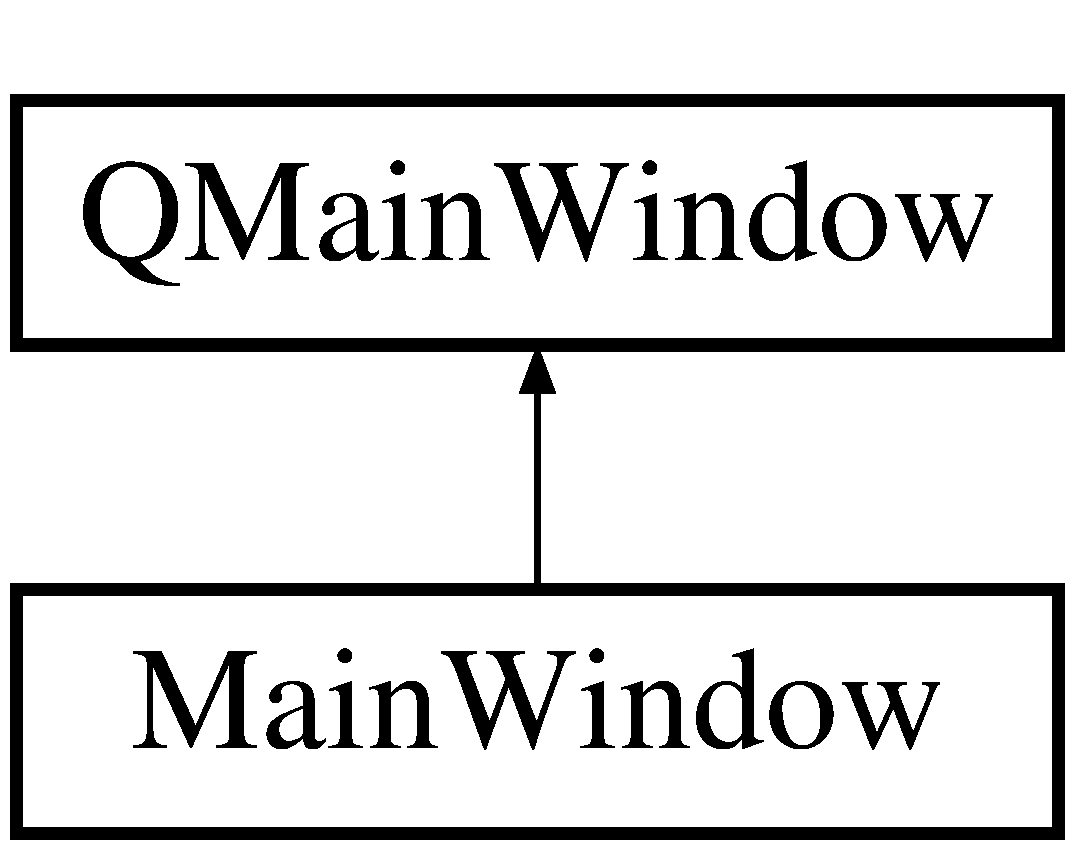
\includegraphics[height=2.000000cm]{classMainWindow}
\end{center}
\end{figure}
\subsection*{Public Member Functions}
\begin{DoxyCompactItemize}
\item 
\hypertarget{classMainWindow_a8b244be8b7b7db1b08de2a2acb9409db}{{\bfseries Main\-Window} (Q\-Widget $\ast$parent=0)}\label{classMainWindow_a8b244be8b7b7db1b08de2a2acb9409db}

\end{DoxyCompactItemize}


\subsection{Detailed Description}
this class connects G\-U\-I with \hyperlink{classNGLScene}{N\-G\-L\-Scene} 

The documentation for this class was generated from the following files\-:\begin{DoxyCompactItemize}
\item 
include/\hyperlink{MainWindow_8h}{Main\-Window.\-h}\item 
src/Main\-Window.\-cpp\end{DoxyCompactItemize}

\hypertarget{classNGLScene}{\section{N\-G\-L\-Scene Class Reference}
\label{classNGLScene}\index{N\-G\-L\-Scene@{N\-G\-L\-Scene}}
}


this class draws all elements for the swarming simulation  




{\ttfamily \#include $<$N\-G\-L\-Scene.\-h$>$}

Inheritance diagram for N\-G\-L\-Scene\-:\begin{figure}[H]
\begin{center}
\leavevmode
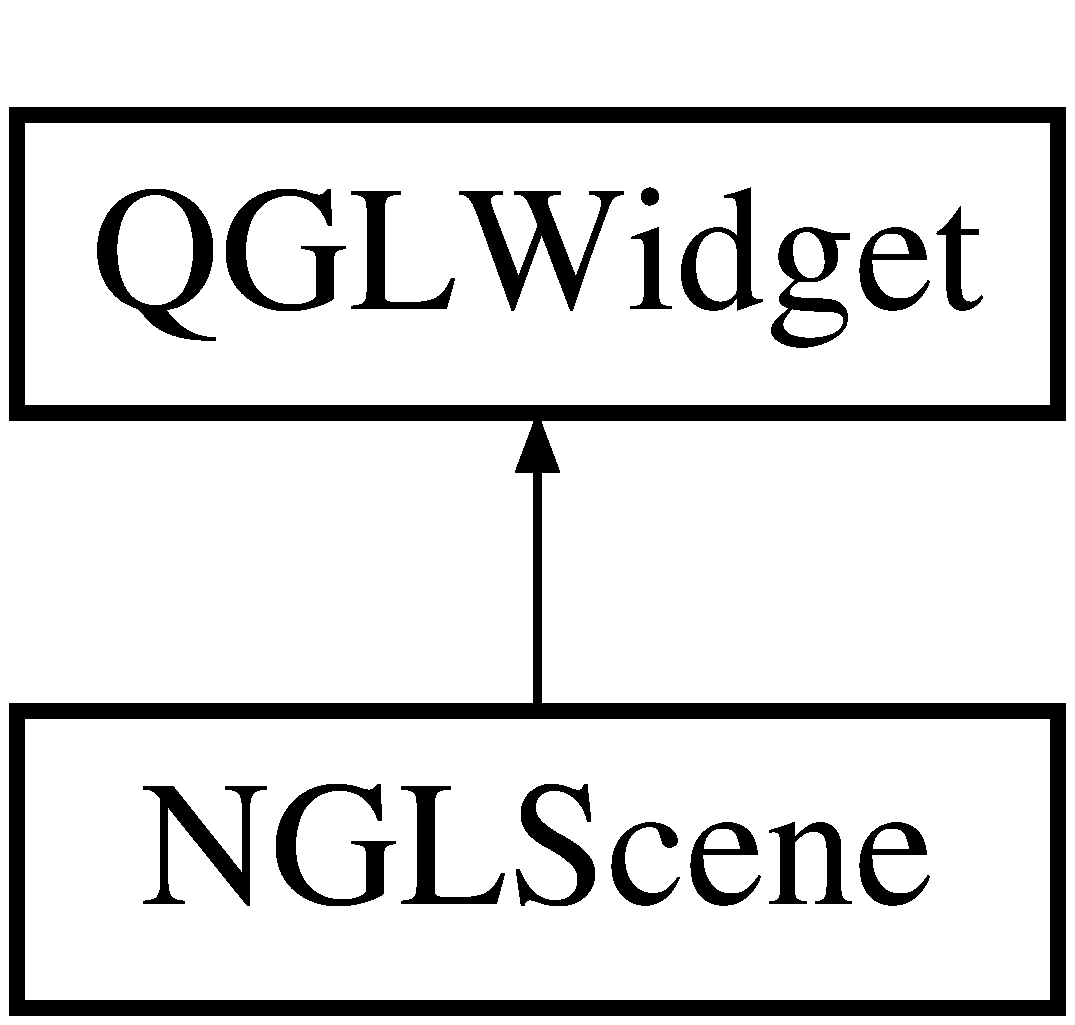
\includegraphics[height=2.000000cm]{classNGLScene}
\end{center}
\end{figure}
\subsection*{Public Slots}
\begin{DoxyCompactItemize}
\item 
\hypertarget{classNGLScene_a8652734544a0635612103759b4ad5cad}{void \hyperlink{classNGLScene_a8652734544a0635612103759b4ad5cad}{remove\-Boid} ()}\label{classNGLScene_a8652734544a0635612103759b4ad5cad}

\begin{DoxyCompactList}\small\item\em A slot to remove a boid. \end{DoxyCompactList}\item 
void \hyperlink{classNGLScene_a5e08b4415869e9c4cf73c49c02f33948}{set\-Cohesion} (int \-\_\-cohesion)
\begin{DoxyCompactList}\small\item\em A slot to set cohesion weight. \end{DoxyCompactList}\item 
void \hyperlink{classNGLScene_af12eae745b8b0f0b199a98ad4eb59d8c}{set\-Separation} (int \-\_\-separation)
\begin{DoxyCompactList}\small\item\em A slot to set separation. \end{DoxyCompactList}\item 
void \hyperlink{classNGLScene_a9f5e5754ca687a66725e5ec05883ec6c}{set\-Alignment} (int \-\_\-align)
\begin{DoxyCompactList}\small\item\em A slot to set alignment. \end{DoxyCompactList}\item 
void \hyperlink{classNGLScene_aeb6a3e90a1db49beef452ca4c3b92de7}{set\-Speed} (int \-\_\-speed)
\begin{DoxyCompactList}\small\item\em A slot to set speed. \end{DoxyCompactList}\item 
void \hyperlink{classNGLScene_a412a3b478a7a2838f6c5096fbbd20095}{set\-Mass} (int \-\_\-mass)
\begin{DoxyCompactList}\small\item\em A slot to set mass. \end{DoxyCompactList}\item 
\hypertarget{classNGLScene_aa25f3abf87cb93d42850b68edbbf6965}{void \hyperlink{classNGLScene_aa25f3abf87cb93d42850b68edbbf6965}{set\-Sep\-Dist} (int \-\_\-sep\-Dist)}\label{classNGLScene_aa25f3abf87cb93d42850b68edbbf6965}

\begin{DoxyCompactList}\small\item\em A slot to set the separation distance for the separation method. \end{DoxyCompactList}\end{DoxyCompactItemize}
\subsection*{Public Member Functions}
\begin{DoxyCompactItemize}
\item 
\hyperlink{classNGLScene_a5c5abd9632cc61aa6bfbb8c237d66f27}{N\-G\-L\-Scene} (Q\-Widget $\ast$\-\_\-parent)
\begin{DoxyCompactList}\small\item\em Constructor for \hyperlink{classNGLScene}{N\-G\-L\-Scene}. \end{DoxyCompactList}\item 
\hypertarget{classNGLScene_abda05d130945833bfbb6bad8d619f7f5}{\hyperlink{classNGLScene_abda05d130945833bfbb6bad8d619f7f5}{$\sim$\-N\-G\-L\-Scene} ()}\label{classNGLScene_abda05d130945833bfbb6bad8d619f7f5}

\begin{DoxyCompactList}\small\item\em dtor \end{DoxyCompactList}\item 
void \hyperlink{classNGLScene_a095aa31c773745194160da96fc5aebe8}{new\-Swarm} (int \-\_\-num\-Boids, int \-\_\-cohesion, int \-\_\-separation, int \-\_\-alignment, float \-\_\-speed, int \-\_\-mass)
\begin{DoxyCompactList}\small\item\em This method is called to create a new swarm. \end{DoxyCompactList}\item 
void \hyperlink{classNGLScene_aace337174f906e2ba944d233c9f4f529}{create\-Swarm} (int \-\_\-cohesion, int \-\_\-separation, int \-\_\-alignment, float \-\_\-speed, int \-\_\-mass)
\begin{DoxyCompactList}\small\item\em A method to add a boid. \end{DoxyCompactList}\end{DoxyCompactItemize}
\subsection*{Protected Member Functions}
\begin{DoxyCompactItemize}
\item 
\hypertarget{classNGLScene_aab2b866db534d286a56cc2240ed98790}{void \hyperlink{classNGLScene_aab2b866db534d286a56cc2240ed98790}{initialize\-G\-L} ()}\label{classNGLScene_aab2b866db534d286a56cc2240ed98790}

\begin{DoxyCompactList}\small\item\em The following methods must be implimented in the sub class this is called when the window is created //-\/-\/-\/-\/-\/-\/-\/-\/-\/-\/-\/-\/-\/-\/-\/-\/-\/-\/-\/-\/-\/-\/-\/-\/-\/-\/-\/-\/-\/-\/-\/-\/-\/-\/-\/-\/-\/-\/-\/-\/-\/-\/-\/-\/-\/-\/-\/-\/-\/-\/-\/-\/-\/-\/-\/-\/-\/-\/-\/-\/-\/-\/-\/-\/-\/-\/-\/-\/-\/-\/-\/-\/-\/-\/-\/-\/-\/-\/-\/-\/-\/-\/-\/-\/-\/-\/-\/-\/-\/-\/-\/-\/-\/-\/-\/-\/-\/-\/-\/-\/-\/-\/-\/-\/-\/-\/-\/-\/-\/-\/-\/-\/---. \end{DoxyCompactList}\item 
void \hyperlink{classNGLScene_ad08cff2eb790203c04862aee6e5432bd}{resize\-G\-L} (const int \-\_\-w, const int \-\_\-h)
\begin{DoxyCompactList}\small\item\em this is called whenever the window is re-\/sized \end{DoxyCompactList}\item 
\hypertarget{classNGLScene_a37bec65bfba7b7a717d803d369221e2d}{void \hyperlink{classNGLScene_a37bec65bfba7b7a717d803d369221e2d}{paint\-G\-L} ()}\label{classNGLScene_a37bec65bfba7b7a717d803d369221e2d}

\begin{DoxyCompactList}\small\item\em this is the main gl drawing routine which is called whenever the window needs to \end{DoxyCompactList}\end{DoxyCompactItemize}


\subsection{Detailed Description}
this class draws all elements for the swarming simulation 

\subsection{Constructor \& Destructor Documentation}
\hypertarget{classNGLScene_a5c5abd9632cc61aa6bfbb8c237d66f27}{\index{N\-G\-L\-Scene@{N\-G\-L\-Scene}!N\-G\-L\-Scene@{N\-G\-L\-Scene}}
\index{N\-G\-L\-Scene@{N\-G\-L\-Scene}!NGLScene@{N\-G\-L\-Scene}}
\subsubsection[{N\-G\-L\-Scene}]{\setlength{\rightskip}{0pt plus 5cm}N\-G\-L\-Scene\-::\-N\-G\-L\-Scene (
\begin{DoxyParamCaption}
\item[{Q\-Widget $\ast$}]{\-\_\-parent}
\end{DoxyParamCaption}
)}}\label{classNGLScene_a5c5abd9632cc61aa6bfbb8c237d66f27}


Constructor for \hyperlink{classNGLScene}{N\-G\-L\-Scene}. 


\begin{DoxyParams}[1]{Parameters}
\mbox{\tt in}  & {\em \-\_\-parent} & the parent window to create the G\-L context in \\
\hline
\end{DoxyParams}


\subsection{Member Function Documentation}
\hypertarget{classNGLScene_aace337174f906e2ba944d233c9f4f529}{\index{N\-G\-L\-Scene@{N\-G\-L\-Scene}!create\-Swarm@{create\-Swarm}}
\index{create\-Swarm@{create\-Swarm}!NGLScene@{N\-G\-L\-Scene}}
\subsubsection[{create\-Swarm}]{\setlength{\rightskip}{0pt plus 5cm}void N\-G\-L\-Scene\-::create\-Swarm (
\begin{DoxyParamCaption}
\item[{int}]{\-\_\-cohesion, }
\item[{int}]{\-\_\-separation, }
\item[{int}]{\-\_\-alignment, }
\item[{float}]{\-\_\-speed, }
\item[{int}]{\-\_\-mass}
\end{DoxyParamCaption}
)}}\label{classNGLScene_aace337174f906e2ba944d233c9f4f529}


A method to add a boid. 


\begin{DoxyParams}[1]{Parameters}
\mbox{\tt in}  & {\em \-\_\-cohesion} & the cohesion weight to set \\
\hline
\mbox{\tt in}  & {\em \-\_\-separation} & the separation weight to set \\
\hline
\mbox{\tt in}  & {\em \-\_\-alignment} & the alignment weight to set \\
\hline
\mbox{\tt in}  & {\em \-\_\-speed} & the speed value to set \\
\hline
\mbox{\tt in}  & {\em \-\_\-mass} & the mass value to set \\
\hline
\end{DoxyParams}
\hypertarget{classNGLScene_a095aa31c773745194160da96fc5aebe8}{\index{N\-G\-L\-Scene@{N\-G\-L\-Scene}!new\-Swarm@{new\-Swarm}}
\index{new\-Swarm@{new\-Swarm}!NGLScene@{N\-G\-L\-Scene}}
\subsubsection[{new\-Swarm}]{\setlength{\rightskip}{0pt plus 5cm}void N\-G\-L\-Scene\-::new\-Swarm (
\begin{DoxyParamCaption}
\item[{int}]{\-\_\-num\-Boids, }
\item[{int}]{\-\_\-cohesion, }
\item[{int}]{\-\_\-separation, }
\item[{int}]{\-\_\-alignment, }
\item[{float}]{\-\_\-speed, }
\item[{int}]{\-\_\-mass}
\end{DoxyParamCaption}
)}}\label{classNGLScene_a095aa31c773745194160da96fc5aebe8}


This method is called to create a new swarm. 


\begin{DoxyParams}[1]{Parameters}
\mbox{\tt in}  & {\em \-\_\-num\-Boids} & the numder of boinds in the new swarm \\
\hline
\mbox{\tt in}  & {\em \-\_\-cohesion} & the cohesion weight to set to each boid \\
\hline
\mbox{\tt in}  & {\em \-\_\-separation} & the separation weight to set to each boid \\
\hline
\mbox{\tt in}  & {\em \-\_\-alignment} & the alignment weight to set to each boid \\
\hline
\mbox{\tt in}  & {\em \-\_\-speed} & the speed value to set to each boid \\
\hline
\mbox{\tt in}  & {\em \-\_\-mass} & the mass value to set to each boid \\
\hline
\end{DoxyParams}
\hypertarget{classNGLScene_ad08cff2eb790203c04862aee6e5432bd}{\index{N\-G\-L\-Scene@{N\-G\-L\-Scene}!resize\-G\-L@{resize\-G\-L}}
\index{resize\-G\-L@{resize\-G\-L}!NGLScene@{N\-G\-L\-Scene}}
\subsubsection[{resize\-G\-L}]{\setlength{\rightskip}{0pt plus 5cm}void N\-G\-L\-Scene\-::resize\-G\-L (
\begin{DoxyParamCaption}
\item[{const int}]{\-\_\-w, }
\item[{const int}]{\-\_\-h}
\end{DoxyParamCaption}
)\hspace{0.3cm}{\ttfamily [protected]}}}\label{classNGLScene_ad08cff2eb790203c04862aee6e5432bd}


this is called whenever the window is re-\/sized 


\begin{DoxyParams}[1]{Parameters}
\mbox{\tt in}  & {\em \-\_\-w} & the width of the resized window \\
\hline
\mbox{\tt in}  & {\em \-\_\-h} & the height of the resized window \\
\hline
\end{DoxyParams}
\hypertarget{classNGLScene_a9f5e5754ca687a66725e5ec05883ec6c}{\index{N\-G\-L\-Scene@{N\-G\-L\-Scene}!set\-Alignment@{set\-Alignment}}
\index{set\-Alignment@{set\-Alignment}!NGLScene@{N\-G\-L\-Scene}}
\subsubsection[{set\-Alignment}]{\setlength{\rightskip}{0pt plus 5cm}void N\-G\-L\-Scene\-::set\-Alignment (
\begin{DoxyParamCaption}
\item[{int}]{\-\_\-align}
\end{DoxyParamCaption}
)\hspace{0.3cm}{\ttfamily [slot]}}}\label{classNGLScene_a9f5e5754ca687a66725e5ec05883ec6c}


A slot to set alignment. 


\begin{DoxyParams}[1]{Parameters}
\mbox{\tt in}  & {\em \-\_\-align} & the value to set \\
\hline
\end{DoxyParams}
\hypertarget{classNGLScene_a5e08b4415869e9c4cf73c49c02f33948}{\index{N\-G\-L\-Scene@{N\-G\-L\-Scene}!set\-Cohesion@{set\-Cohesion}}
\index{set\-Cohesion@{set\-Cohesion}!NGLScene@{N\-G\-L\-Scene}}
\subsubsection[{set\-Cohesion}]{\setlength{\rightskip}{0pt plus 5cm}void N\-G\-L\-Scene\-::set\-Cohesion (
\begin{DoxyParamCaption}
\item[{int}]{\-\_\-cohesion}
\end{DoxyParamCaption}
)\hspace{0.3cm}{\ttfamily [slot]}}}\label{classNGLScene_a5e08b4415869e9c4cf73c49c02f33948}


A slot to set cohesion weight. 


\begin{DoxyParams}[1]{Parameters}
\mbox{\tt in}  & {\em \-\_\-cohesion} & the value to set \\
\hline
\end{DoxyParams}
\hypertarget{classNGLScene_a412a3b478a7a2838f6c5096fbbd20095}{\index{N\-G\-L\-Scene@{N\-G\-L\-Scene}!set\-Mass@{set\-Mass}}
\index{set\-Mass@{set\-Mass}!NGLScene@{N\-G\-L\-Scene}}
\subsubsection[{set\-Mass}]{\setlength{\rightskip}{0pt plus 5cm}void N\-G\-L\-Scene\-::set\-Mass (
\begin{DoxyParamCaption}
\item[{int}]{\-\_\-mass}
\end{DoxyParamCaption}
)\hspace{0.3cm}{\ttfamily [slot]}}}\label{classNGLScene_a412a3b478a7a2838f6c5096fbbd20095}


A slot to set mass. 


\begin{DoxyParams}[1]{Parameters}
\mbox{\tt in}  & {\em \-\_\-mass} & the value to set \\
\hline
\end{DoxyParams}
\hypertarget{classNGLScene_af12eae745b8b0f0b199a98ad4eb59d8c}{\index{N\-G\-L\-Scene@{N\-G\-L\-Scene}!set\-Separation@{set\-Separation}}
\index{set\-Separation@{set\-Separation}!NGLScene@{N\-G\-L\-Scene}}
\subsubsection[{set\-Separation}]{\setlength{\rightskip}{0pt plus 5cm}void N\-G\-L\-Scene\-::set\-Separation (
\begin{DoxyParamCaption}
\item[{int}]{\-\_\-separation}
\end{DoxyParamCaption}
)\hspace{0.3cm}{\ttfamily [slot]}}}\label{classNGLScene_af12eae745b8b0f0b199a98ad4eb59d8c}


A slot to set separation. 


\begin{DoxyParams}[1]{Parameters}
\mbox{\tt in}  & {\em \-\_\-separation} & the value to set \\
\hline
\end{DoxyParams}
\hypertarget{classNGLScene_aeb6a3e90a1db49beef452ca4c3b92de7}{\index{N\-G\-L\-Scene@{N\-G\-L\-Scene}!set\-Speed@{set\-Speed}}
\index{set\-Speed@{set\-Speed}!NGLScene@{N\-G\-L\-Scene}}
\subsubsection[{set\-Speed}]{\setlength{\rightskip}{0pt plus 5cm}void N\-G\-L\-Scene\-::set\-Speed (
\begin{DoxyParamCaption}
\item[{int}]{\-\_\-speed}
\end{DoxyParamCaption}
)\hspace{0.3cm}{\ttfamily [slot]}}}\label{classNGLScene_aeb6a3e90a1db49beef452ca4c3b92de7}


A slot to set speed. 


\begin{DoxyParams}[1]{Parameters}
\mbox{\tt in}  & {\em \-\_\-speed} & the value to set \\
\hline
\end{DoxyParams}


The documentation for this class was generated from the following files\-:\begin{DoxyCompactItemize}
\item 
include/\hyperlink{NGLScene_8h}{N\-G\-L\-Scene.\-h}\item 
src/N\-G\-L\-Scene.\-cpp\end{DoxyCompactItemize}

\hypertarget{classOctree}{\section{Octree Class Reference}
\label{classOctree}\index{Octree@{Octree}}
}


I have used this class for finding the neighbours of a boid in my swarming system. I have made small modification from the original class such as removing methods which were not necesarrily needed for the calculations.  




{\ttfamily \#include $<$Octree.\-h$>$}

\subsection*{Public Member Functions}
\begin{DoxyCompactItemize}
\item 
\hyperlink{classOctree_a18c97528102fc6c7b0afcf62d4256d6b}{Octree} (ngl\-::\-Vec3 \-\_\-origin, float \-\_\-half\-D, int \-\_\-height)
\begin{DoxyCompactList}\small\item\em ctor \end{DoxyCompactList}\item 
\hypertarget{classOctree_a6705a6ae06fab5a0dfdd79f45576020d}{\hyperlink{classOctree_a6705a6ae06fab5a0dfdd79f45576020d}{$\sim$\-Octree} ()}\label{classOctree_a6705a6ae06fab5a0dfdd79f45576020d}

\begin{DoxyCompactList}\small\item\em dtor recursivley destroys octants \end{DoxyCompactList}\item 
void \hyperlink{classOctree_a5e902807821df11683179aea5e43d731}{set\-Data} (ngl\-::\-Vec4 \-\_\-data)
\begin{DoxyCompactList}\small\item\em sets the m\-\_\-data member variable \end{DoxyCompactList}\item 
int \hyperlink{classOctree_adb4be848e01fce3568b83cd8a4117e26}{get\-Octant\-Containing\-Point} (ngl\-::\-Vec3 point)
\begin{DoxyCompactList}\small\item\em Determine which octant of the tree contains \char`\"{}point\char`\"{}. \end{DoxyCompactList}\item 
bool \hyperlink{classOctree_a5311ba068ebb82dbc917e0178f052ec0}{is\-Leaf} ()
\begin{DoxyCompactList}\small\item\em checks whether the current node is a leaf node \end{DoxyCompactList}\item 
void \hyperlink{classOctree_a9a1092104eeea9725e66ae188b8db736}{insert} (ngl\-::\-Vec4 \-\_\-data)
\begin{DoxyCompactList}\small\item\em if this node doesnt have a data point; insert one or if is does; split this node into 8 children and insert old and new data points \end{DoxyCompactList}\item 
ngl\-::\-Vec4 \hyperlink{classOctree_a814ed4196b414829c44f55c8b65a7517}{get\-Points\-Inside\-Sphere} (ngl\-::\-Vec3 centre, float radius)
\begin{DoxyCompactList}\small\item\em query the tree for points within a bounding sphere \end{DoxyCompactList}\item 
\hypertarget{classOctree_aca0adcb1047b4ced99f1e3449ac88036}{void \hyperlink{classOctree_aca0adcb1047b4ced99f1e3449ac88036}{clear\-Results} ()}\label{classOctree_aca0adcb1047b4ced99f1e3449ac88036}

\begin{DoxyCompactList}\small\item\em resets m\-\_\-results\-Data \end{DoxyCompactList}\item 
\hypertarget{classOctree_a6ac1e8420a5b02c854e8ebcf8e18a401}{void \hyperlink{classOctree_a6ac1e8420a5b02c854e8ebcf8e18a401}{build\-V\-A\-O} ()}\label{classOctree_a6ac1e8420a5b02c854e8ebcf8e18a401}

\begin{DoxyCompactList}\small\item\em builds a simple V\-A\-O object of the octrree for visualisation purposes \end{DoxyCompactList}\end{DoxyCompactItemize}
\subsection*{Public Attributes}
\begin{DoxyCompactItemize}
\item 
\hypertarget{classOctree_a6260225ce5323751e8053cfd4597f2cd}{std\-::vector$<$ ngl\-::\-Vec4 $>$ \hyperlink{classOctree_a6260225ce5323751e8053cfd4597f2cd}{m\-\_\-results\-Data}}\label{classOctree_a6260225ce5323751e8053cfd4597f2cd}

\begin{DoxyCompactList}\small\item\em resets m\-\_\-results\-Data \end{DoxyCompactList}\end{DoxyCompactItemize}


\subsection{Detailed Description}
I have used this class for finding the neighbours of a boid in my swarming system. I have made small modification from the original class such as removing methods which were not necesarrily needed for the calculations. 

\subsection{Constructor \& Destructor Documentation}
\hypertarget{classOctree_a18c97528102fc6c7b0afcf62d4256d6b}{\index{Octree@{Octree}!Octree@{Octree}}
\index{Octree@{Octree}!Octree@{Octree}}
\subsubsection[{Octree}]{\setlength{\rightskip}{0pt plus 5cm}Octree\-::\-Octree (
\begin{DoxyParamCaption}
\item[{ngl\-::\-Vec3}]{\-\_\-origin, }
\item[{float}]{\-\_\-half\-D, }
\item[{int}]{\-\_\-height}
\end{DoxyParamCaption}
)}}\label{classOctree_a18c97528102fc6c7b0afcf62d4256d6b}


ctor 


\begin{DoxyParams}[1]{Parameters}
\mbox{\tt in}  & {\em \-\_\-origin} & the physical centre of the node \\
\hline
\mbox{\tt in}  & {\em \-\_\-half\-D} & half the width, depth, or height of the node \\
\hline
\mbox{\tt in}  & {\em \-\_\-height} & the height of the octree \\
\hline
\end{DoxyParams}


\subsection{Member Function Documentation}
\hypertarget{classOctree_adb4be848e01fce3568b83cd8a4117e26}{\index{Octree@{Octree}!get\-Octant\-Containing\-Point@{get\-Octant\-Containing\-Point}}
\index{get\-Octant\-Containing\-Point@{get\-Octant\-Containing\-Point}!Octree@{Octree}}
\subsubsection[{get\-Octant\-Containing\-Point}]{\setlength{\rightskip}{0pt plus 5cm}int Octree\-::get\-Octant\-Containing\-Point (
\begin{DoxyParamCaption}
\item[{ngl\-::\-Vec3}]{point}
\end{DoxyParamCaption}
)}}\label{classOctree_adb4be848e01fce3568b83cd8a4117e26}


Determine which octant of the tree contains \char`\"{}point\char`\"{}. 


\begin{DoxyParams}[1]{Parameters}
\mbox{\tt in}  & {\em point} & the point to check \\
\hline
\end{DoxyParams}
\begin{DoxyReturn}{Returns}
int denoting the octant containing \char`\"{}point\char`\"{} 
\end{DoxyReturn}
\hypertarget{classOctree_a814ed4196b414829c44f55c8b65a7517}{\index{Octree@{Octree}!get\-Points\-Inside\-Sphere@{get\-Points\-Inside\-Sphere}}
\index{get\-Points\-Inside\-Sphere@{get\-Points\-Inside\-Sphere}!Octree@{Octree}}
\subsubsection[{get\-Points\-Inside\-Sphere}]{\setlength{\rightskip}{0pt plus 5cm}ngl\-::\-Vec4 Octree\-::get\-Points\-Inside\-Sphere (
\begin{DoxyParamCaption}
\item[{ngl\-::\-Vec3}]{centre, }
\item[{float}]{radius}
\end{DoxyParamCaption}
)}}\label{classOctree_a814ed4196b414829c44f55c8b65a7517}


query the tree for points within a bounding sphere 


\begin{DoxyParams}[1]{Parameters}
\mbox{\tt in}  & {\em centre} & the centre of the bounding sphere \\
\hline
\mbox{\tt in}  & {\em radius} & the radius of the bounding sphere \\
\hline
\end{DoxyParams}
\begin{DoxyReturn}{Returns}
returns and appends the points inside the bounding sphere to m\-\_\-results\-Data 
\end{DoxyReturn}
\hypertarget{classOctree_a9a1092104eeea9725e66ae188b8db736}{\index{Octree@{Octree}!insert@{insert}}
\index{insert@{insert}!Octree@{Octree}}
\subsubsection[{insert}]{\setlength{\rightskip}{0pt plus 5cm}void Octree\-::insert (
\begin{DoxyParamCaption}
\item[{ngl\-::\-Vec4}]{\-\_\-data}
\end{DoxyParamCaption}
)}}\label{classOctree_a9a1092104eeea9725e66ae188b8db736}


if this node doesnt have a data point; insert one or if is does; split this node into 8 children and insert old and new data points 


\begin{DoxyParams}[1]{Parameters}
\mbox{\tt in}  & {\em \-\_\-data} & the data to insert \\
\hline
\end{DoxyParams}
\hypertarget{classOctree_a5311ba068ebb82dbc917e0178f052ec0}{\index{Octree@{Octree}!is\-Leaf@{is\-Leaf}}
\index{is\-Leaf@{is\-Leaf}!Octree@{Octree}}
\subsubsection[{is\-Leaf}]{\setlength{\rightskip}{0pt plus 5cm}bool Octree\-::is\-Leaf (
\begin{DoxyParamCaption}
{}
\end{DoxyParamCaption}
)}}\label{classOctree_a5311ba068ebb82dbc917e0178f052ec0}


checks whether the current node is a leaf node 

\begin{DoxyReturn}{Returns}
true if node is leaf or false if not 
\end{DoxyReturn}
\hypertarget{classOctree_a5e902807821df11683179aea5e43d731}{\index{Octree@{Octree}!set\-Data@{set\-Data}}
\index{set\-Data@{set\-Data}!Octree@{Octree}}
\subsubsection[{set\-Data}]{\setlength{\rightskip}{0pt plus 5cm}void Octree\-::set\-Data (
\begin{DoxyParamCaption}
\item[{ngl\-::\-Vec4}]{\-\_\-data}
\end{DoxyParamCaption}
)}}\label{classOctree_a5e902807821df11683179aea5e43d731}


sets the m\-\_\-data member variable 


\begin{DoxyParams}[1]{Parameters}
\mbox{\tt in}  & {\em \-\_\-data} & the data to assign to m\-\_\-data \\
\hline
\end{DoxyParams}


The documentation for this class was generated from the following files\-:\begin{DoxyCompactItemize}
\item 
include/\hyperlink{Octree_8h}{Octree.\-h}\item 
src/Octree.\-cpp\end{DoxyCompactItemize}

\hypertarget{classSwarm}{\section{Swarm Class Reference}
\label{classSwarm}\index{Swarm@{Swarm}}
}


a class for creating the swarm, managing boids and their neighbours  




{\ttfamily \#include $<$Swarm.\-h$>$}

\subsection*{Public Member Functions}
\begin{DoxyCompactItemize}
\item 
\hyperlink{classSwarm_af3423d580972ffbe9a1b7befb8d75caf}{Swarm} (int \-\_\-num\-Boids)
\begin{DoxyCompactList}\small\item\em ctor \end{DoxyCompactList}\item 
\hyperlink{classSwarm_ac2a239ad48e9d468b8d6de0f321dbabb}{Swarm} (int \-\_\-num\-Boids, int \-\_\-cohesion, int \-\_\-separation, int \-\_\-alignment, float \-\_\-speed, int \-\_\-mass)
\begin{DoxyCompactList}\small\item\em ctor to set custom steering force weights, speed and mass as well as the number of boids \end{DoxyCompactList}\item 
\hypertarget{classSwarm_a5d74bf7e768edf0d8930ba187005a583}{\hyperlink{classSwarm_a5d74bf7e768edf0d8930ba187005a583}{$\sim$\-Swarm} ()}\label{classSwarm_a5d74bf7e768edf0d8930ba187005a583}

\begin{DoxyCompactList}\small\item\em dtor \end{DoxyCompactList}\item 
void \hyperlink{classSwarm_aaf270a2467917858d8f8a636c04783e7}{create\-Swarm} (int \-\_\-cohesion, int \-\_\-separation, int \-\_\-alignment, float \-\_\-speed, int \-\_\-mass)
\begin{DoxyCompactList}\small\item\em method to add a boid to the swarm \end{DoxyCompactList}\item 
\hypertarget{classSwarm_a69fc2af93e0ec34bdcd309f34e7be3ab}{void \hyperlink{classSwarm_a69fc2af93e0ec34bdcd309f34e7be3ab}{remove\-Boid} ()}\label{classSwarm_a69fc2af93e0ec34bdcd309f34e7be3ab}

\begin{DoxyCompactList}\small\item\em method to remove a boid from the swarm \end{DoxyCompactList}\item 
void \hyperlink{classSwarm_a2edf4a7143b520b4390e2f7fe948c843}{set\-Neighbours} (int \-\_\-id)
\begin{DoxyCompactList}\small\item\em method to st the boid position \end{DoxyCompactList}\item 
\hypertarget{classSwarm_a21bce2e4048f0ed95f91544069d4a009}{int \hyperlink{classSwarm_a21bce2e4048f0ed95f91544069d4a009}{get\-Size} ()}\label{classSwarm_a21bce2e4048f0ed95f91544069d4a009}

\begin{DoxyCompactList}\small\item\em method to return the size of the swarm \end{DoxyCompactList}\item 
\hypertarget{classSwarm_adae7b2b5b76d18fe5c3d3118515b48c9}{void \hyperlink{classSwarm_adae7b2b5b76d18fe5c3d3118515b48c9}{update\-Swarm} ()}\label{classSwarm_adae7b2b5b76d18fe5c3d3118515b48c9}

\begin{DoxyCompactList}\small\item\em method to update the swarm, neighbours, collisions and positions of the boids \end{DoxyCompactList}\end{DoxyCompactItemize}
\subsection*{Public Attributes}
\begin{DoxyCompactItemize}
\item 
\hypertarget{classSwarm_a43829aa093ffd59ebc2c759667674428}{std\-::vector$<$ \hyperlink{classBoid}{Boid} $>$ \hyperlink{classSwarm_a43829aa093ffd59ebc2c759667674428}{m\-\_\-swarm}}\label{classSwarm_a43829aa093ffd59ebc2c759667674428}

\begin{DoxyCompactList}\small\item\em vector to contain all boids within the swarm \end{DoxyCompactList}\end{DoxyCompactItemize}


\subsection{Detailed Description}
a class for creating the swarm, managing boids and their neighbours 

\subsection{Constructor \& Destructor Documentation}
\hypertarget{classSwarm_af3423d580972ffbe9a1b7befb8d75caf}{\index{Swarm@{Swarm}!Swarm@{Swarm}}
\index{Swarm@{Swarm}!Swarm@{Swarm}}
\subsubsection[{Swarm}]{\setlength{\rightskip}{0pt plus 5cm}Swarm\-::\-Swarm (
\begin{DoxyParamCaption}
\item[{int}]{\-\_\-num\-Boids}
\end{DoxyParamCaption}
)}}\label{classSwarm_af3423d580972ffbe9a1b7befb8d75caf}


ctor 


\begin{DoxyParams}[1]{Parameters}
\mbox{\tt in}  & {\em \-\_\-num\-Boids} & the number of boids in the swarm \\
\hline
\end{DoxyParams}
\hypertarget{classSwarm_ac2a239ad48e9d468b8d6de0f321dbabb}{\index{Swarm@{Swarm}!Swarm@{Swarm}}
\index{Swarm@{Swarm}!Swarm@{Swarm}}
\subsubsection[{Swarm}]{\setlength{\rightskip}{0pt plus 5cm}Swarm\-::\-Swarm (
\begin{DoxyParamCaption}
\item[{int}]{\-\_\-num\-Boids, }
\item[{int}]{\-\_\-cohesion, }
\item[{int}]{\-\_\-separation, }
\item[{int}]{\-\_\-alignment, }
\item[{float}]{\-\_\-speed, }
\item[{int}]{\-\_\-mass}
\end{DoxyParamCaption}
)}}\label{classSwarm_ac2a239ad48e9d468b8d6de0f321dbabb}


ctor to set custom steering force weights, speed and mass as well as the number of boids 


\begin{DoxyParams}[1]{Parameters}
\mbox{\tt in}  & {\em \-\_\-num\-Boids} & the number of boids in the swarm \\
\hline
\mbox{\tt in}  & {\em \-\_\-cohesion} & the custom cohesion force weight to set \\
\hline
\mbox{\tt in}  & {\em \-\_\-separation} & the custom spearation force weight to set \\
\hline
\mbox{\tt in}  & {\em \-\_\-alignment} & the custom alignment force weight to set \\
\hline
\mbox{\tt in}  & {\em \-\_\-speed} & the custom speed value to be set \\
\hline
\mbox{\tt in}  & {\em \-\_\-mass} & the custom mass value to be set \\
\hline
\end{DoxyParams}


\subsection{Member Function Documentation}
\hypertarget{classSwarm_aaf270a2467917858d8f8a636c04783e7}{\index{Swarm@{Swarm}!create\-Swarm@{create\-Swarm}}
\index{create\-Swarm@{create\-Swarm}!Swarm@{Swarm}}
\subsubsection[{create\-Swarm}]{\setlength{\rightskip}{0pt plus 5cm}void Swarm\-::create\-Swarm (
\begin{DoxyParamCaption}
\item[{int}]{\-\_\-cohesion, }
\item[{int}]{\-\_\-separation, }
\item[{int}]{\-\_\-alignment, }
\item[{float}]{\-\_\-speed, }
\item[{int}]{\-\_\-mass}
\end{DoxyParamCaption}
)}}\label{classSwarm_aaf270a2467917858d8f8a636c04783e7}


method to add a boid to the swarm 


\begin{DoxyParams}[1]{Parameters}
\mbox{\tt in}  & {\em \-\_\-cohesion} & the cohesion force weight to set to the boid \\
\hline
\mbox{\tt in}  & {\em \-\_\-separation} & the spearation force weight to set to the boid \\
\hline
\mbox{\tt in}  & {\em \-\_\-alignment} & the alignment force weight to set to the boid \\
\hline
\mbox{\tt in}  & {\em \-\_\-speed} & the speed value to set to the boid \\
\hline
\mbox{\tt in}  & {\em \-\_\-mass} & the mass value to set to the boid \\
\hline
\end{DoxyParams}
\hypertarget{classSwarm_a2edf4a7143b520b4390e2f7fe948c843}{\index{Swarm@{Swarm}!set\-Neighbours@{set\-Neighbours}}
\index{set\-Neighbours@{set\-Neighbours}!Swarm@{Swarm}}
\subsubsection[{set\-Neighbours}]{\setlength{\rightskip}{0pt plus 5cm}void Swarm\-::set\-Neighbours (
\begin{DoxyParamCaption}
\item[{int}]{\-\_\-id}
\end{DoxyParamCaption}
)}}\label{classSwarm_a2edf4a7143b520b4390e2f7fe948c843}


method to st the boid position 


\begin{DoxyParams}[1]{Parameters}
\mbox{\tt in}  & {\em \-\_\-id} & the id of the boid to set neighbours to \\
\hline
\end{DoxyParams}


The documentation for this class was generated from the following files\-:\begin{DoxyCompactItemize}
\item 
include/\hyperlink{Swarm_8h}{Swarm.\-h}\item 
src/Swarm.\-cpp\end{DoxyCompactItemize}

\chapter{File Documentation}
\hypertarget{Boid_8h}{\section{include/\-Boid.h File Reference}
\label{Boid_8h}\index{include/\-Boid.\-h@{include/\-Boid.\-h}}
}
{\ttfamily \#include $<$ctime$>$}\\*
{\ttfamily \#include $<$deque$>$}\\*
{\ttfamily \#include $<$iostream$>$}\\*
{\ttfamily \#include $<$ngl/\-Vertex\-Array\-Object.\-h$>$}\\*
{\ttfamily \#include $<$ngl/\-Transformation.\-h$>$}\\*
{\ttfamily \#include $<$ngl/\-Vec3.\-h$>$}\\*
{\ttfamily \#include $<$stdlib.\-h$>$}\\*
{\ttfamily \#include $<$vector$>$}\\*
\subsection*{Classes}
\begin{DoxyCompactItemize}
\item 
class \hyperlink{classBoid}{Boid}
\begin{DoxyCompactList}\small\item\em this class contains movement methods and behaviours for the boids \end{DoxyCompactList}\end{DoxyCompactItemize}

\hypertarget{BoidMath_8h}{\section{include/\-Boid\-Math.h File Reference}
\label{BoidMath_8h}\index{include/\-Boid\-Math.\-h@{include/\-Boid\-Math.\-h}}
}
{\ttfamily \#include $<$math.\-h$>$}\\*
{\ttfamily \#include $<$ngl/\-Vec3.\-h$>$}\\*
{\ttfamily \#include $<$ngl/\-Vec2.\-h$>$}\\*
{\ttfamily \#include $<$ngl/\-Mat4.\-h$>$}\\*
{\ttfamily \#include $<$vector$>$}\\*
\subsection*{Classes}
\begin{DoxyCompactItemize}
\item 
class \hyperlink{classBoidMath}{Boid\-Math}
\begin{DoxyCompactList}\small\item\em this class calculates the distance between the boids \end{DoxyCompactList}\end{DoxyCompactItemize}

\hypertarget{MainWindow_8h}{\section{include/\-Main\-Window.h File Reference}
\label{MainWindow_8h}\index{include/\-Main\-Window.\-h@{include/\-Main\-Window.\-h}}
}
{\ttfamily \#include $<$Q\-Main\-Window$>$}\\*
{\ttfamily \#include $<$N\-G\-L\-Scene.\-h$>$}\\*
\subsection*{Classes}
\begin{DoxyCompactItemize}
\item 
class \hyperlink{classMainWindow}{Main\-Window}
\begin{DoxyCompactList}\small\item\em this class connects G\-U\-I with \hyperlink{classNGLScene}{N\-G\-L\-Scene} \end{DoxyCompactList}\end{DoxyCompactItemize}

\hypertarget{NGLScene_8h}{\section{include/\-N\-G\-L\-Scene.h File Reference}
\label{NGLScene_8h}\index{include/\-N\-G\-L\-Scene.\-h@{include/\-N\-G\-L\-Scene.\-h}}
}


a basic Qt G\-L window class for creating a swarming simulation  


{\ttfamily \#include $<$ngl/\-Camera.\-h$>$}\\*
{\ttfamily \#include $<$ngl/\-Transformation.\-h$>$}\\*
{\ttfamily \#include $<$ngl/\-Colour.\-h$>$}\\*
{\ttfamily \#include $<$ngl/\-Light.\-h$>$}\\*
{\ttfamily \#include $<$ngl/\-Shader\-Lib.\-h$>$}\\*
{\ttfamily \#include $<$ngl/\-V\-A\-O\-Primitives.\-h$>$}\\*
{\ttfamily \#include $<$Q\-Event$>$}\\*
{\ttfamily \#include $<$Q\-Resize\-Event$>$}\\*
{\ttfamily \#include $<$Q\-G\-L\-Widget$>$}\\*
{\ttfamily \#include $<$ngl/\-Text.\-h$>$}\\*
{\ttfamily \#include $<$Qt\-Open\-G\-L$>$}\\*
{\ttfamily \#include $<$Swarm.\-h$>$}\\*
\subsection*{Classes}
\begin{DoxyCompactItemize}
\item 
class \hyperlink{classNGLScene}{N\-G\-L\-Scene}
\begin{DoxyCompactList}\small\item\em this class draws all elements for the swarming simulation \end{DoxyCompactList}\end{DoxyCompactItemize}


\subsection{Detailed Description}
a basic Qt G\-L window class for creating a swarming simulation 
\hypertarget{Octree_8h}{\section{include/\-Octree.h File Reference}
\label{Octree_8h}\index{include/\-Octree.\-h@{include/\-Octree.\-h}}
}
{\ttfamily \#include $<$stdlib.\-h$>$}\\*
{\ttfamily \#include $<$ngl/\-Vertex\-Array\-Object.\-h$>$}\\*
{\ttfamily \#include $<$vector$>$}\\*
{\ttfamily \#include $<$ngl/\-Vec4.\-h$>$}\\*
{\ttfamily \#include $<$ngl/\-Vec3.\-h$>$}\\*
\subsection*{Classes}
\begin{DoxyCompactItemize}
\item 
class \hyperlink{classOctree}{Octree}
\begin{DoxyCompactList}\small\item\em I have used this class for finding the neighbours of a boid in my swarming system. I have made small modification from the original class such as removing methods which were not necesarrily needed for the calculations. \end{DoxyCompactList}\end{DoxyCompactItemize}


\subsection{Detailed Description}
Modified from\-: Alexander la Tourelle,Flock Available from\-: \href{https://github.com/mainConfetti/Flock}{\tt https\-://github.\-com/main\-Confetti/\-Flock} \mbox{[}online\mbox{]} 
\hypertarget{Swarm_8h}{\section{include/\-Swarm.h File Reference}
\label{Swarm_8h}\index{include/\-Swarm.\-h@{include/\-Swarm.\-h}}
}
{\ttfamily \#include $<$stdlib.\-h$>$}\\*
{\ttfamily \#include $<$cmath$>$}\\*
{\ttfamily \#include $<$vector$>$}\\*
{\ttfamily \#include $<$Boid.\-h$>$}\\*
{\ttfamily \#include $<$Octree.\-h$>$}\\*
\subsection*{Classes}
\begin{DoxyCompactItemize}
\item 
class \hyperlink{classSwarm}{Swarm}
\begin{DoxyCompactList}\small\item\em a class for creating the swarm, managing boids and their neighbours \end{DoxyCompactList}\end{DoxyCompactItemize}

%--- End generated contents ---

% Index
\newpage
\phantomsection
\addcontentsline{toc}{part}{Index}
\printindex

\end{document}
